\documentclass[a4paper,
fontsize=11pt,
%headings=small,
oneside,
numbers=noperiodatend,
parskip=half-,
bibliography=totoc,
final
]{scrartcl}

\usepackage{synttree}
\usepackage{graphicx}
\setkeys{Gin}{width=.4\textwidth} %default pics size

\graphicspath{{./plots/}}
\usepackage[ngerman]{babel}
\usepackage[T1]{fontenc}
%\usepackage{amsmath}
\usepackage[utf8x]{inputenc}
\usepackage [hyphens]{url}
\usepackage{booktabs} 
\usepackage[left=2.4cm,right=2.4cm,top=2.3cm,bottom=2cm,includeheadfoot]{geometry}
\usepackage{eurosym}
\usepackage{multirow}
\usepackage[ngerman]{varioref}
\setcapindent{1em}
\renewcommand{\labelitemi}{--}
\usepackage{paralist}
\usepackage{pdfpages}
\usepackage{lscape}
\usepackage{float}
\usepackage{acronym}
\usepackage{eurosym}
\usepackage[babel]{csquotes}
\usepackage{longtable,lscape}
\usepackage{mathpazo}
\usepackage[normalem]{ulem} %emphasize weiterhin kursiv
\usepackage[flushmargin,ragged]{footmisc} % left align footnote
\usepackage{ccicons} 
\usepackage{afterpage}

%%%% fancy LIBREAS URL color 
\usepackage{xcolor}
\definecolor{libreas}{RGB}{112,0,0}

\usepackage{listings}

\urlstyle{same}  % don't use monospace font for urls

\usepackage[fleqn]{amsmath}

%adjust fontsize for part

\usepackage{sectsty}
\partfont{\large}

%Das BibTeX-Zeichen mit \BibTeX setzen:
\def\symbol#1{\char #1\relax}
\def\bsl{{\tt\symbol{'134}}}
\def\BibTeX{{\rm B\kern-.05em{\sc i\kern-.025em b}\kern-.08em
    T\kern-.1667em\lower.7ex\hbox{E}\kern-.125emX}}

\usepackage{fancyhdr}
\fancyhf{}
\pagestyle{fancyplain}
\fancyhead[R]{\thepage}

% make sure bookmarks are created eventough sections are not numbered!
% uncommend if sections are numbered (bookmarks created by default)
\makeatletter
\renewcommand\@seccntformat[1]{}
\makeatother


\usepackage{hyperxmp}
\usepackage[colorlinks, linkcolor=black,citecolor=black, urlcolor=libreas,
breaklinks= true,bookmarks=true,bookmarksopen=true]{hyperref}
%URLs hart brechen
\makeatletter 
\g@addto@macro\UrlBreaks{ 
  \do\a\do\b\do\c\do\d\do\e\do\f\do\g\do\h\do\i\do\j 
  \do\k\do\l\do\m\do\n\do\o\do\p\do\q\do\r\do\s\do\t 
  \do\u\do\v\do\w\do\x\do\y\do\z\do\&\do\1\do\2\do\3 
  \do\4\do\5\do\6\do\7\do\8\do\9\do\0} 
% \def\do@url@hyp{\do\-} 
\makeatother 

%meta
%meta

\fancyhead[L]{S. Dogunke, T. Steyer, C. Mayer \\ %author
LIBREAS. Library Ideas, 33 (2018). % journal, issue, volume.
\href{http://nbn-resolving.de/}
{}} % urn 
% recommended use
%\href{http://nbn-resolving.de/}{\color{black}{urn:nbn:de...}}
\fancyhead[R]{\thepage} %page number
\fancyfoot[L] {\ccLogo \ccAttribution\ \href{https://creativecommons.org/licenses/by/3.0/}{\color{black}Creative Commons BY 3.0}}  %licence
\fancyfoot[R] {ISSN: 1860-7950}

\title{\LARGE{Barcamp Data and Demons: von Bestands- und Forschungsdaten zu Services \\
Treffen sich ein Bibliothekar, eine Archäologin, ein Informatiker, …}} % title
\author{Swantje Dogunke, Timo Steyer, Corinna Mayer} % author

\setcounter{page}{1}

\hypersetup{%
      pdftitle={Barcamp Data and Demons: von Bestands- und Forschungsdaten zu Services},
      pdfauthor={Swantje Dogunke, Timo Steyer, Corinna Mayer},
      pdfcopyright={CC BY 3.0 Unported},
      pdfsubject={LIBREAS. Library Ideas, 33 (2018).},
      pdfkeywords={Barcamp, Forschungsdaten, Digital Humanities, Forschungsverbund Marbach Weimar Wolfenbüttel},
      pdflicenseurl={https://creativecommons.org/licenses/by/3.0/},
      pdfcontacturl={http://libreas.eu},
      baseurl={http://libreas.eu},
      pdflang={de},
      pdfmetalang={de}
     }



\date{}
\begin{document}

\maketitle
\thispagestyle{fancyplain} 

%abstracts
\begin{abstract}
Der Beitrag thematisiert das innovative Tagungsformat eines Barcamps am
konkreten Beispiel der im Rahmen des Forschungsverbundes Marbach Weimar
Wolfenbüttel durchgeführten Veranstaltung ``Data and Demons: Von
Bestanddaten zu Services''. Ziel war es, Vertreter/innen der
verschiedenen Fachdisziplinen an Bibliotheken, Archiven und Museen
zusammenzubringen, die im Feld der Digital Humanities arbeiten. Das
kommunikative Format stellt Veranstalter/innen und Teilnehmer/innen vor
neue Herausforderungen, eignet sich jedoch dank der agilen
Agendaentwicklung dafür, rasch neue Perspektiven auf bestandsbezogene
Forschung an Bibliotheken zu entwickeln und Impulse für die Digital
Humanities zu generieren. Einen guten Einstieg bot die Keynote von Ralf
Stockmann in der Herzog August Bibliothek Wolfenbüttel mit dem Titel
``Der Zauberlehrling war nicht als Anleitung gemeint'' über Künstliche
Intelligenz in Kultur- und Wissenschaftseinrichtungen.\\

The article broaches the issue of the conference format of a Barcamp
using the event Data and Demons: From Collections' Data to Services as
example. The event, held by the Research Association Marbach Weimar
Wolfenbüttel, aims to bring together scientists of various disciplines
who work in the field of Digital Humanities at libraries, archives und
museums. The participatory format of the event presents both hosts and
participants with new challenges and opportunities. Due to the
self-organizing nature of a Barcamp, the participants develop new
perspectives on collection-based research in libraries and create
momentum for the Digital Humanities. The keynote by Ralf Stockmann, for
example, offered an excellent introduction to Artificial Intelligence in
scientific and cultural institutions.
\end{abstract}

%body
\begin{center}\rule{0.5\linewidth}{\linethickness}\end{center}

Der Forschungsverbund Marbach Weimar Wolfenbüttel (MWW) empfing diese
und 49 andere interessierte Expert/innen ihres Faches vom 27. bis 28.
November 2017 zu einem ersten Digital-Humanities-Barcamp an der Herzog
August Bibliothek in Wolfenbüttel. Die Ziele waren hoch gesteckt: Es
sollten aktuelle Fragestellungen und Probleme der Digital Humanities im
Kontext von Kulturerbeinstitutionen und Informatik diskutiert werden.
Der Weg einer klassischen Tagung sollte bewusst nicht beschritten
werden, um die unterschiedlichen Disziplinen zusammenzubringen. Es
musste ein kommunikatives und freies Format gefunden werden -- die Wahl
fiel auf das offene Tagungsformat \enquote{Barcamp}.

Während 2017 bereits das zehnte BibCamp -- ein Barcamp mit
bibliothekarischen Schwerpunkten -- stattfand,\footnote{Veranstaltungswebsite:
  \url{https://bibcamp.wordpress.com/}.} ist die Ausrichtung eines
Barcamps im Bereich der Digital Humanities und der Geisteswissenschaften
bisher eher ungewöhnlich. Allerdings verbreitet sich diese im
angloamerikanischen Raum schon etablierte Form langsam auch im
geisteswissenschaftlichen Kontext, wie Veranstaltungen wie das
histocamp, einem Barcamp für Geschichtsinteressierte, belegen.\footnote{Vgl.
  \url{https://www.histocamp.de/}.}

Die wichtigsten Erfolgsfaktoren für ein Gelingen eines DH-Barcamps sind
die vielfältige Zusammensetzung der Teilnehmer/innen, ein
Kommunikationskonzept, die Räumlichkeiten und äußeren Bedingungen, eine
offene Einstellung zu möglichen Ergebnissen sowie Teilnehmer/innen, die
sich auf ein solch ungewöhnliches Vorhaben einlassen.\footnote{Hilfreiche
  weitere Faktoren bietet der von L. Azzimonti, Marzia A. Cremona,
  Andrea Ghiglietti, et al.~entwickelte Algorithmus in: BarCamp:
  Technology Foresight and Statistics for the Future, 2014. S. 55.}

\hypertarget{organisation-und-vorbereitungen}{%
\section{Organisation und
Vorbereitungen}\label{organisation-und-vorbereitungen}}

Die Herzog August Bibliothek als Veranstaltungsort verfügt über eigene
Tagungsräume und personelle Ressourcen für die Organisation von
wissenschaftlichen Veranstaltungen, jedoch stellte das neue Format trotz
der günstigen Voraussetzungen die Organisatoren/innen vor neue
Herausforderungen.

Auch für viele Teilnehmer/innen stellte die Veranstaltung \enquote{Data
and Demons} das erste Barcamp dar, was zu einem erhöhten
Kommunikationsaufwand in der Vorbereitung führte. Es bestand
Klärungsbedarf in Fragen der Themenvorbereitung, des Ablaufes und der
konkreten Durchführung. Irritierend wirkte vor allem der Ablaufplan, der
keine konkreten Themen beinhaltet, da diese erst im Rahmen der agilen
Agendaentwicklung konkretisiert werden sollen.\footnote{Vgl. das
  Tagungsprogramm unter:
  \url{http://www.mww-forschung.de/fileadmin/user_upload/_imported/fileadmin/user_upload/MWW/Veranstaltungen/Programm_Barcamp171102.pdf}.}
Um über das Format zu informieren wurde ein Beitrag zum Thema
\enquote{Was ist ein Barcamp} im Blog des Forschungsverbundes MWW
publiziert.\footnote{Vgl. Moritz Avenarius: Barcamp \enquote{Data and
  Demons: Von Bestands- UND Forschungsdaten zu Services}. Online:
  \url{http://www.mww-forschung.de/blog/blogdetail/barcamp-data-and-demons-von-bestands-und-forschungsdaten-zu-services-im-rahmen-des-forschungsverbunds-mww}
  {[}Stand: 8.12.2017{]}.}

Anstatt eines großen Tagungsraums wurden drei kleinere Seminarräume und
die Cafeteria als Veranstaltungsorte ausgewählt, um parallele Sessions
zu ermöglichen. Es wurde Moderationsmaterial bereitgestellt und ein
Kommunikationskanal über Twitter eingerichtet,\footnote{Über
  \url{https://twitter.com/data_demons} sowie über die Hashtags
  \href{https://twitter.com/hashtag/mww?src=hash}{\#mww}
  \href{https://twitter.com/hashtag/dhbarcamp?src=hash}{\#dhbarcamp}
  kann der Verlauf der Veranstaltung und auch die Reaktion der
  Teilnehmer/innen nachvollzogen werden.} da eine vorherige Analyse
ergab, dass etwa zwei Drittel der Teilnehmer einen Twitteraccount
pflegen.\footnote{Vgl. dazu auch die Ausführungen im Abschnitt
  \enquote{Kommunikation}.}

Damit die Tagungsteilnehmer/innen schon vor dem Beginn des eigentlichen
Barcamps thematisch an das Thema \enquote{Data and Demons} herangeführt
werden konnten, wurde beschlossen eine Keynote und einen Empfang am
Abend vor Beginn der Veranstaltung durchzuführen. Die Keynote sollte als
\emph{Opener} dienen, aber auch Vorbehalte gegenüber dem unbekannten
Format am kommenden Tag abbauen und ein erstes Kennenlernen der
Teilnehmer/innen ermöglichen.

\hypertarget{die-teilnehmerinnen}{%
\section{Die Teilnehmer/innen}\label{die-teilnehmerinnen}}

Die Veranstaltung war für jede/n Interessierte/n offen, eine gezielte
Ansprache einiger der insgesamt 52 Teilnehmer/innen erfolgte jedoch im
Vorfeld, um ein Gleichgewicht der Disziplinen und Stakeholder und eine
Vielfalt an akademischen Graden zu erreichen.\footnote{Circa die Hälfte
  der Teilnehmer/innen war vor Beginn der Veranstaltung eingeladen
  worden, während die andere Hälfte durch die Bekanntgabe der
  Veranstaltung über Blogs, Twitter und Veranstaltungshinweise auf den
  Homepages der beteiligten Einrichtungen auf das Barcamp aufmerksam
  wurde.} Die Maxime für eine Veranstaltung dieser Art ist: Jede/r ist
Experte/in seines/ihres Faches und kann Sessionvorschläge einbringen.
Auf diese Weise entstand eine über verschiedene Fachdisziplinen
verteilte Teilnehmer/innen/gruppe, die Studenten/innen ebenso umfasste
wie Lehrstuhlinhaber/innen oder Bibliothekare/innen. Die Mehrzahl der
Teilnehmer/innen war dem Feld Digital Humanities zuzuordnen, wobei diese
Gruppe sich weniger aus dem universitären Kontext als vielmehr aus
wissenschaftlichen Bibliotheken zusammensetzte. Der überwiegende Teil
der Teilnehmer/innen verfügte über mehrjährige DH-Projekterfahrungen und
hatte einen geisteswissenschaftlichen Hintergrund.

\hypertarget{die-kommunikation}{%
\section{Die Kommunikation}\label{die-kommunikation}}

Während der Vorbereitungen wurde die Entscheidung getroffen einen
externen Experten mit der Moderation des Barcamps zu beauftragen. Die
Aufgaben des Moderators sind vorab zu klären, in diesem Fall waren es
die Einführung, die Moderation der Agendaentwicklung und der
Ergebnispräsentation sowie das Zeitmanagement während der Veranstaltung.
Die Wahl fiel auf den Hamburger Moderator Moritz Avenarius, der bereits
Barcamps zu ähnlichen Themen erfolgreich moderiert hat.\footnote{\url{http://www.zukunftslotse.de/}.}

Das Barcamp wurde auch selbst zum Forschungsgegenstand: Der Virtuelle
Forschungsraum des MWW wurde erstmals eingesetzt, um den Bedarf an
digitaler Infrastruktur für die Durchführung eines Barcamps zu
untersuchen. Er diente als zentraler Einstieg, um Informationen zur
Veranstaltung für die Teilnehmer/innen und Interessierten in einem
öffentlichen Bereich zu präsentieren.\footnote{\url{https://vfr.mww-forschung.de/web/barcamp-data-and-demons}.}
Eine vorherige Analyse ergab, wie schon gesagt, dass etwa zwei Drittel
der Teilnehmer/innen aktiv einen Twitteraccount pflegen. Um auch die
anderen Teilnehmer/innen über die Twitter-Aktivitäten zu informieren,
wurden die Timelines im Virtuellen Forschungsraum angezeigt.

\begin{figure}
\centering
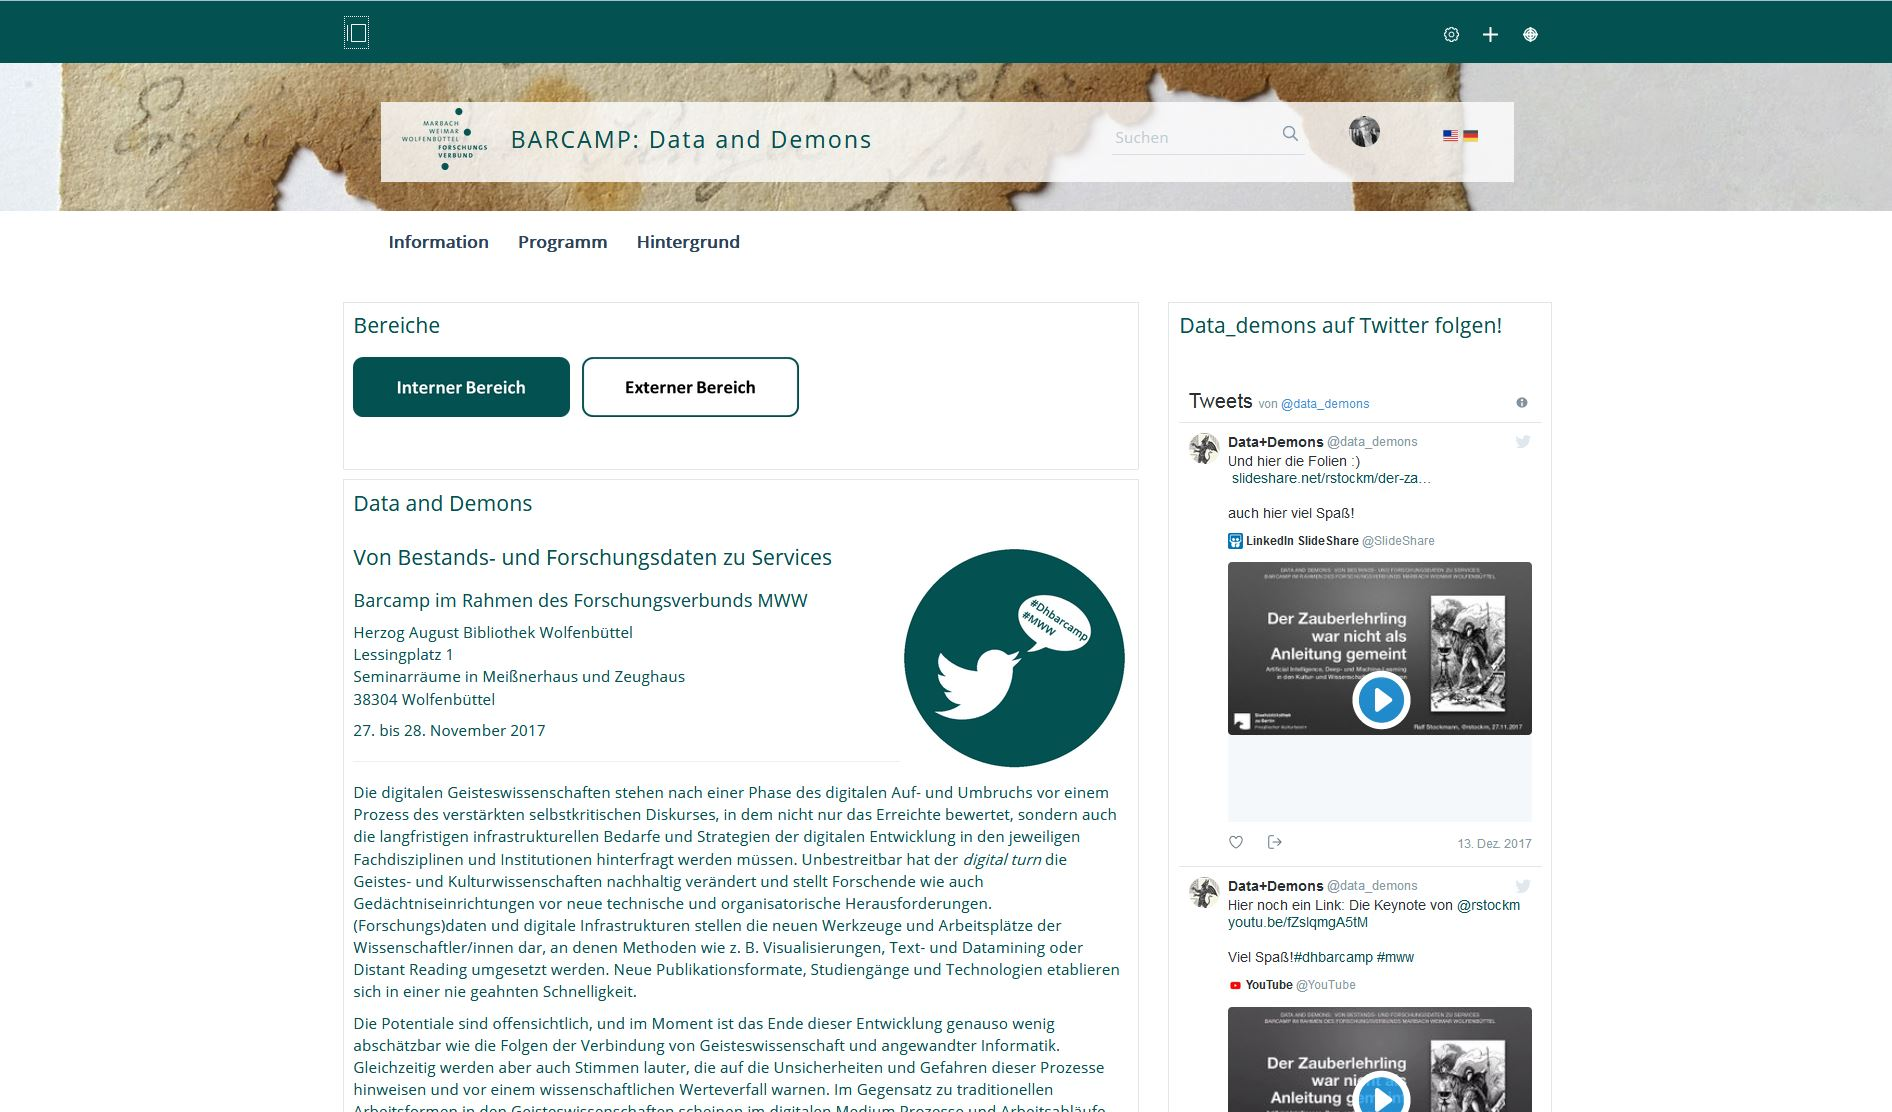
\includegraphics[width=0.7\columnwidth]{img/Abbildung1.jpg}
\caption{Screenshot des Virtuellen Forschungsraums MWW mit dem Auftritt
zum Barcamp.}
\end{figure}

Der private Bereich des Virtuellen Forschungsraums bietet die
Möglichkeit, \emph{Etherpads} anzulegen und zu nutzen, um
Sessionvorschläge im Vorfeld und während der Veranstaltung mitzuteilen,
sowie Ergebnisse und Diskussionen festzuhalten. Eine
Teilnehmer/innen/liste und die Möglichkeit, sich direkt mit anderen
Teilnehmer/innen auszutauschen, waren weitere Angebote im privaten
Bereich des Virtuellen Forschungsraumes.\footnote{Ungenutzt blieb ein
  anonymer digitaler \enquote{Kummerkasten}.}

Die Pflege des Twitterkanals während der Veranstaltung übernahm eine
studentische Hilfskraft. Ziel war es, Nicht-Teilnehmende über die
Aktivitäten und Diskussionen zu informieren und einzubinden.\footnote{Auch
  im Vorfeld konnten Sessionvorschläge über Twitter adressiert werden.}
Zudem wurde Twitter genutzt, um Planänderungen, zeitliche Verschiebungen
und zusätzliche Informationen an die Teilnehmer/innen zu adressieren.
Auch wenn die bereits erwähnte Analyse ergab, dass nur zwei Drittel der
Teilnehmer/innen Twitter aktiv nutzen, konnten diese als
Multiplikator/innen während des Veranstaltung dienen, um alle
Beteiligten zu erreichen.

\hypertarget{ruxe4umlichkeiten-und-uxe4uuxdfere-bedingungen}{%
\section{Räumlichkeiten und äußere
Bedingungen}\label{ruxe4umlichkeiten-und-uxe4uuxdfere-bedingungen}}

Für ein Barcamp wird ein zentraler Raum benötigt, in dem sich die
Teilnehmer/innen zusammenfinden und die agile Planung der Veranstaltung
durchführen können. Je nach Menge der Sessionvorschläge bedarf es
weiterer Räume für die parallele Durchführung von Sessions.

\afterpage{
\begin{figure}
\centering
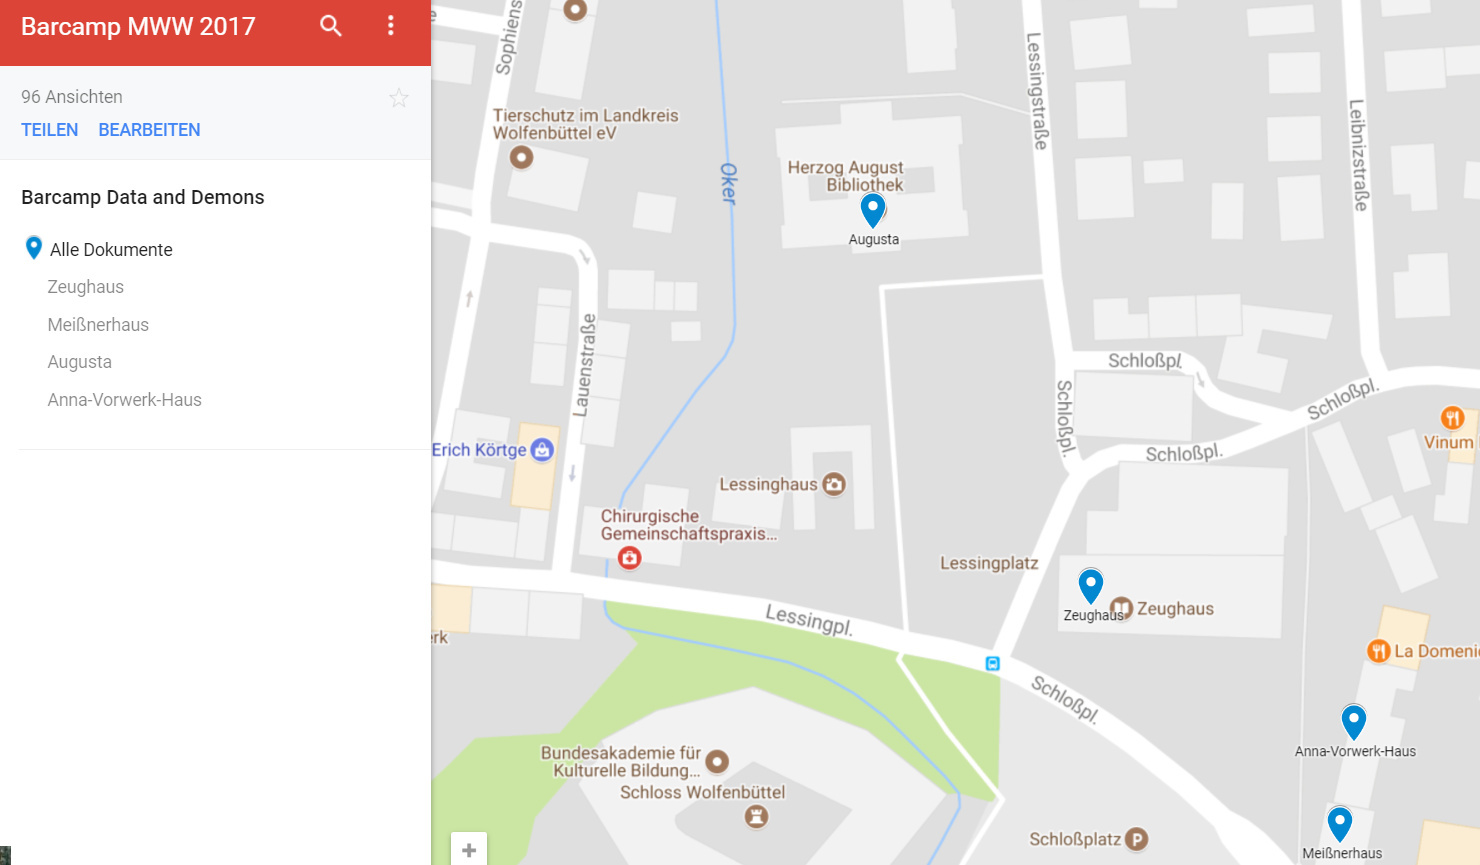
\includegraphics[width=0.7\columnwidth]{img/Abbildung2.jpg}
\caption{Verteilung der Seminarräume auf das Wolfenbütteler Bibliotheksquartier.\footnotemark}
\end{figure}
\footnotetext{Vgl. \href{https://www.google.de/maps/@52.1622099,10.5375103,15z?hl=de\&authuser=0}{https://www.google.de/maps/@52.1622099,10.5375103,15z?hl=de\&authuser=0}}
}

In Wolfenbüttel waren drei Seminarräume vorhanden. Zusätzlich erwies
sich die Nutzung der Cafeteria als Ort für kleinere Gesprächsrunden, die
auf sehr spezielle Fragen konzentriert waren, als gewinnbringend. In der
Cafeteria wurde später auch das Sessionboard aufgestellt, auf dem Themen
der Sessions, die Orte und Uhrzeiten festgehalten waren. So konnte die
Hemmschwelle der Teilnahme für regulär arbeitende Wissenschaftler/innen
und Bibliothekare/innen zumindest teilweise überwunden werden, da eine
Teilnahme für einzelne Sessions möglich war. Da Twitter als ein
zentrales Kommunikationsformat genutzt wurde, war das Vorhandensein von
WLAN obligatorisch. Moderationsmaterial wurde benötigt, um die
Diskussion und die Ergebnisse der Sessions anzuleiten beziehungsweise zu
dokumentieren.

\hypertarget{die-keynote-als-impuls}{%
\section{Die Keynote als Impuls}\label{die-keynote-als-impuls}}

Die von Ralf Stockmann (Staatsbibliothek zu Berlin -- Preußischer
Kulturbesitz) gehaltene Keynote mit dem Titel \enquote{Der
Zauberlehrling war nicht als Anleitung gemeint. Artificial Intelligence,
Deep- und Machine-Learning in den Kultur- und
Wissenschaftseinrichtungen} gewährte einen Blick in die Zukunft von
wissenschaftlichen Bibliotheken, der angesichts der Potentiale von
künstlicher Intelligenz sowohl begeisternd wie beängstigend
war.\footnote{Eine Videoaufnahme der Keynote ist zu finden unter:
  \url{https://youtu.be/fZslqmgA5tM} Die Folien können eingesehen werden
  unter:
  \url{https://www.slideshare.net/rstockm/der-zauberlehrling-war-nicht-als-anleitung-gemeint-83960825}}
Der Kontrast zwischen dem digitalen Thema des Vortrages, verbunden mit
dem Einsatz moderner Medien zu der im Hintergrund angestrahlten
historischen Büchersammlung des 17. Jahrhunderts, schuf eine ideale
Kulisse für die Frage nach der zukünftigen Rolle von Bibliotheken in
einer digitalen beziehungsweise sich digitalisierenden Welt. Die sich an
den Vortrag anschließenden Diskussionen zeigten bereits, dass dieses
Thema sowohl Geisteswissenschaftler/innen als auch Bibliothekare/innen
und Informatiker/innen anspricht und auf unterschiedlichen Ebenen
beschäftigt. Das Thema der Keynote und die sich daran anschließenden
Gespräche waren nicht nur ein guter Einstieg für das Barcamp, sondern
brachten Ideen und Vorschläge zu Sessions hervor, die am nächsten Tag
aufgegriffen wurden. Die Impulse der Keynote zeigten die Potentiale und
die sich daraus entwickelnde Diskussionsdynamik auf, welche durch die
oben beschriebene Divergenz von Digtialem und historischem Bestand
hervorgebracht wurde.

\begin{figure}
\centering
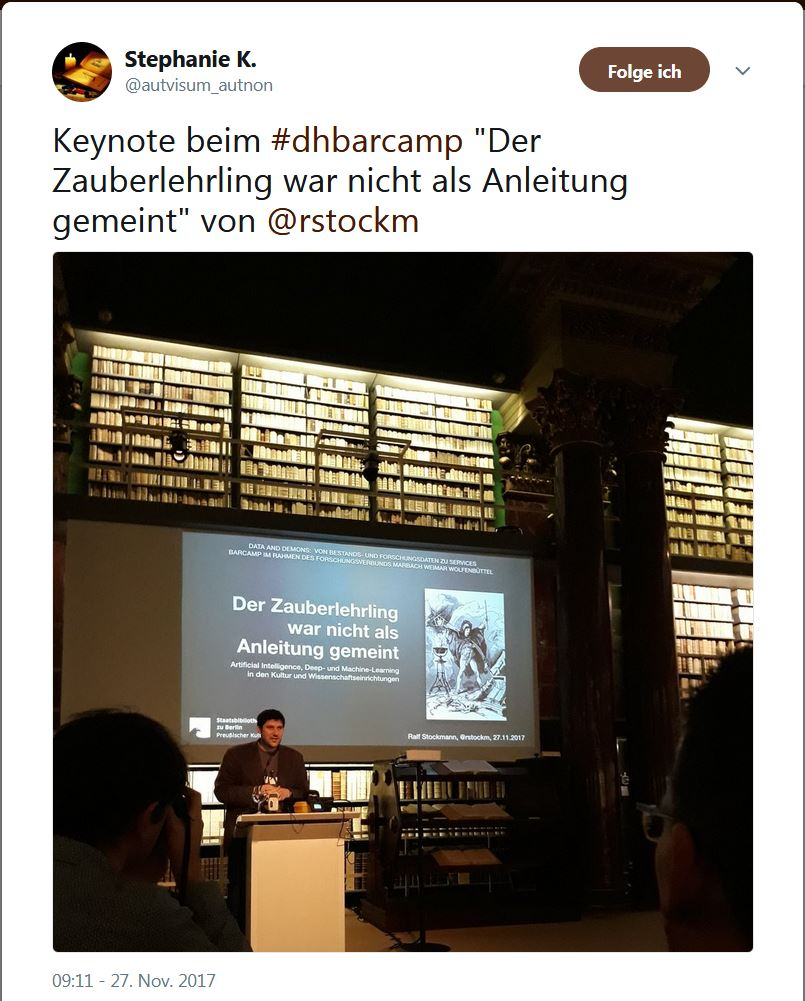
\includegraphics{img/Abbildung3.jpg}
\caption{Tweet von @autvisum\_autnon vom 27. November 2017. Online:
\href{https://twitter.com/autvisum\_autnon/status/935194297950928897}{https://twitter.com/autvisum\_autnon/status/935194297950928897}}
\end{figure}

\hypertarget{einfuxfchrung-und-beginn}{%
\section{Einführung und Beginn}\label{einfuxfchrung-und-beginn}}

Das eigentliche Barcamp begann am Morgen des zweiten Tages. Nach einer
Begrüßung und Einführung in das Format der Veranstaltung nannte der
Moderator die Regeln für das Barcamp. So empfahl er, dass sich im Rahmen
der Veranstaltung die Beteiligten duzen, die Sessions wurden als offene
Veranstaltungen deklariert und die zentralen Punkte jeder Session
sollten auf Kapaplatten (Kunstschaumplatten) festgehalten und später
allen Teilnehmer/innen präsentiert werden. Im Anschluss stellten sich
alle Teilnehmer/innen kurz vor, wobei sie drei Hashtags angaben, die ihr
fachliches Profil umreißen sollten. Anhand dieser Profile gab es zum
\enquote{Aufwärmen} offene Kommunikationsrunden, in welchen sich jeweils
zu zweit und in wechselnden Konstellationen über die eigenen Erwartungen
und Wünsche an das Barcamp ausgetauscht wurde. Hier erwies sich die
offene und im Raum verteilte Kommunikation als sehr inspirierend, da die
Anzahl der Teilnehmer/innen in dem kleinen Raum eine bienenstockartige
Atmosphäre schuf. Dieses Vorgehen kreierte eine gute Grundlage für den
nächsten Schritt: das Einbringen von Sessionvorschlägen im Rahmen der
agilen Planung.

\hypertarget{die-themen-sessions}{%
\section{Die Themen / Sessions}\label{die-themen-sessions}}

Als Einzelperson oder in kleineren Gruppen wurden die Sessionvorschläge
erarbeitet und auf einem Blatt festgehalten. Insgesamt wurden 17
Vorschläge eingebracht. Anschließend wurde jeder Vorschlag durch einen
der Einreichenden präsentiert. Nach der Präsentation wurde um eine kurze
Einschätzung gebeten, wie viele der Teilnehmer/innen sich für die
vorgeschlagene Session interessieren würden. Es entwickelte sich eine
intensive Abstimmungsphase, in der auch Sessionvorschläge zusammengelegt
und entsprechend der Anzahl der interessierten Teilnehmer/innen auf die
unterschiedlichen Räume der Veranstaltungen verteilt wurden. Während für
die größeren Sessions Seminarräume verwendet wurden, bot die Cafeteria
Raum für kleinere Diskussionsrunden.

Die vorgeschlagenen Sessions zeichneten sich durch eine große
Themenvielfalt aus, die methodische ebenso wie theoretische Fragen
umfasst, außerdem wurden Sessions zu konkreten Problemen eingereicht.

% Please add the following required packages to your document preamble:
% \usepackage{booktabs}
\begin{table}[h]
\centering
\footnotesize
\begin{tabular}{p{1.5cm}p{3cm}p{3cm}p{3cm}p{3cm}}
\toprule
 & \textbf{Seminarraum Zeughaus} & \textbf{Meißnerhaus 1} & \textbf{Meißnerhaus 2} & \textbf{Cafeteria} \\
 \midrule
10:30–11:45 & Ich liebe Tabellen – ich hasse Tabellen. Swantje Dogunke & Visionen und Dämonen. Constanze Baum & Automatische Erschließung. Christian Scharfe & Ist DH eine Wissenschaft? Torsten Schassan \\
\midrule
11:30–12:30 & Keine Websites mehr! Daten statt Oberflächen. Fabian Cremer & Was ist eigentlich eine DH-Fragestellung? Benjamin Hübbe & Verhältnis DH / Hermeneutik. Stefan Höppner & Demons sind Freunde. Nils Reichert \\
\midrule
13:30–14:30 & DH: Dienstleistung, Forschung, eierlegende Wollmilchsau. Timo Steyer & Suchen, aber nach was? Andreas Henrich & Haben alle digitalen Editionen einen gemeinsamen Kern? Torsten Schassan & Standardisierung von FRBR in XML/ TEI. Henrike Fricke \\
\midrule
15:00–16:00 & Schuster bleib bei deinen Leisten! Markus Baumgarten & Zitierbarkeit Digitaler Editionen. Martin de la Iglesia, Uwe Sikora, Franziska Diehr & Was ist eigentlich so schwierig am Teilen/Bereitstellen von Forschungsdaten? Lydia Koglin & ~ \\
\bottomrule
\end{tabular}
\caption{Sessionboard mit den vorgeschlagenen Themen.}
\label{tab:1}
\end{table}

Einen besonderer Schwerpunkt beim Barcamp betraf das Selbstverständnis
aber auch die Fremdwahrnehmung der Digital Humanities. Hier ergaben sich
aufgrund des heterogenen Teilnehmerfeldes verschiedene Sichtweisen, aber
auch Teilnehmer/innen aus dem Feld der Digital Humanities
interpretierten ihre Rolle in multidisziplinären Projekten
unterschiedlich. Ein Spannungsverhältnis bestand zum Beispiel in der
Frage, inwieweit der Aufbau und die Entwicklung grundlegender
Forschungsinfrastrukturkomponenten, der Bereich des Digital Consulting
oder die Bereiche der Tool-Anwendung als Forschungsaufgaben deklariert
werden können. Daran anknüpfend wurden die möglichen Rollen der
DH-Forscher/innen in Projektteams skizziert. Selbstkritisch wurde aber
auch von mehreren Beteiligten angemerkt, dass die Digital Humanities zur
Vereinfachung von Problemen neigten und sich selbst durch eine
anfängliche Unterschätzung der Komplexität von technischen Prozessen
unter Zugzwang setzten.

Ein weiteres Themenfeld betraf die Möglichkeit der automatischen
Erschließung von historischen Sammlungen. Die Session näherte sich dem
Thema auf der Grundlage verschiedener Beispiele und
Erschließungsprofile. Dabei wurden vor allem Erfahrungen mit vorhandenen
Tools und semiautomatischen Workflows für die Altbestandserschließung
ausgetauscht und die zentrale Frage diskutiert, inwieweit eine
maschinell gestützte, aber mit Ungenauigkeiten und Fehlern behaftete
Erschließung einen alternativen Weg für die Sammlungsforschung
darstellt. Ist wirklich jede Information besser als keine?

Als ein verbindendes Element und Kommunikationsinstrument der
verschiedenen Fachdisziplinen wurden Tabellen und Listen identifiziert,
da sie seit Jahrhunderten Informationen systematisch verwalten und als
Grundlage für weitere Schritte, wie zum Beispiel der Entwicklung
relationaler Datenbanken, dienen. Die Teilnehmer/innen entwarfen
gemeinsame Anforderungen und empfahlen, in Projekten mit verschiedenen
Disziplinen früh anhand von Tabellen über Forschungsdaten zu reden und
sie als ein niedrigschwelliges Kommunikationsinstrument in
multidisziplinären Forschungsgruppen zu nutzen.

\hypertarget{ergebnisse}{%
\section{Ergebnisse}\label{ergebnisse}}

Nach den Sessions kamen alle Teilnehmer/innen zusammen und präsentierten
den Verlauf und die erzielten Ergebnisse der veranstalteten Sessions. Es
entstand eine intensive Diskussion mit dem Plenum. Die einzelnen
Sessions erzielten ganz unterschiedliche Resultate, die Bandbreite
reichte von der Lösung konkreter Probleme, wie zum Beispiel die
Erstellung eines Vorschlages für die Umsetzung des FRBR-Modells
(Functional Requirements for Bibliographic Records) in XML/TEI, über die
Gründung kleinerer Arbeitsgruppen, die nach dem Barcamp weiterhin an den
Themen arbeiten und auch publizieren wollen, bis zur Konzeption der
Weiterverfolgung eines Sessionthemas in einem eigenen Workshop. Die
Ergebnisse des Barcamps waren freilich sehr heterogen, so dass eine
gemeinsame Ergebnisdokumentation nicht möglich ist. Vielmehr sollen die
geschaffenen Impulse von den Teilnehmer/innen aufgegriffen werden und,
wo es sich anbietet, weitergeführt werden. Viele Teilnehmer/innen sahen
den großen Gewinn in der individuellen Horizonterweiterung und der
Erfahrung, die sie im Rahmen des Barcamps gewonnen hatten.

Alle Teilnehmer/innen waren sich einig, dass sie vom offenen, aktiven
und impulsgebenden Format profitiert haben. Das Barcamp bot jedem
beziehungsweise jeder Einzelnen eine Plattform für die individuelle
Fragestellung. Gerade dieser Raum wurde genutzt, um nicht erneut das
eigene Projekt vorzustellen und zu profilieren, sondern um
Schwachstellen, konkrete Probleme und auch Themen zu erörtern, die nur
schwer auf einer Tagung präsentiert werden können. Dazu gehörten zum
Beispiel Fragen nach der Konzeption und Steuerung von DH-Projekten. Des
Weiteren eignete sich das Format aber auch dazu, stereotypische
Kommunikationsgrenzen einzelner Fachdisziplinen zu überwinden und mit
Expert/innen aus anderen Bereichen intensiv zu diskutieren. Gerade die
heterogene Zusammensetzung wurde als erfolgsrelaventes Kriterium
identifiziert. Aus Sicht der Bibliothek kann festgehalten werden, dass
sich Barcamps eignen, um unterschiedliche Akteurinnen und Akteure der
Einrichtung zusammenzubringen und im Gegensatz zu bibliothekarischen
beziehungsweise wissenschaftlichen Konferenzen stärker Nutzer/innen,
Wissenschaftler/innen und bibliothekarische Mitarbeiter/innen in einen
Dialog bringen zu können.

\hypertarget{resuxfcmee-und-lessons-learned}{%
\section{Resümee und Lessons
learned}\label{resuxfcmee-und-lessons-learned}}

Aus Sicht der Veranstalter/innen überwiegen bei weitem die positiven
Aspekte, auch wenn einige Entscheidungen im Rückblick anders hätten
ausfallen können. Zum einem bedingte die erste Durchführung des Formates
eine gewisse Konzentration des Teilnehmer/innen/kreises, in der
Durchführung erwies sich aber die trotzdem zustande gekommene
Heterogenität als wichtiges Kriterium. Ein gemischtes Teilnehmerfeld
schafft durch das Zusammenbringen unterschiedlicher Perspektiven eine
kontroverse Diskussionskultur. Bei der Gestaltung der Sessionvorschläge
erwiesen sich die Sessions mit konkreten Fragestellungen als die
produktivere Form, so dass stärker auf eine Harmonisierung von problem-,
methodisch- und theorieorientierten Sessions geachtet werden sollte. Ein
geeignetes Mittel wäre die Kategorisierung der Sessions in bestimmte
Kommunikationsstrukturen, wie zum Beispiel Impulsvortrag und Diskussion,
Streitgespräch oder Expert/inn/entische.

Auf der praktischen Ebene sollten die Tagungsräume keine allzu große
räumliche Distanz aufweisen, um das schnelle Wechseln zwischen mehreren
Sessions zu ermöglichen. In der Vorbereitung sollte möglichst früh ein
Kommunikationskanal zu allen Teilnehmer/innen installiert und gepflegt
werden, um Informationen zur Veranstaltung zu verbreiten. Da es sich um
ein sehr konzentriertes Format handelt, welches auch hohe Ansprüche an
die Teilnehmer/innen stellt, sollte die Dauer der Veranstaltung beachtet
werden. Die Zeit für die Vorbereitung eines Barcamps war höher als für
eine traditionelle Veranstaltungsform, zum einen griffen etablierte
Workflows nicht und zum anderen war der Aufwand an Kommunikation mit den
Teilnehmer/innen deutlich höher.

Zusammenfassend liegt der Erfolg eines Barcamps in der Schaffung einer
Atmosphäre, die durch ständige Kommunikation, kritische Diskussionen
aber auch durch Vernetzung und gegenseitigen Respekt geprägt ist.
Klassische Tagungshierarchien zwischen Redner/in und Plenum
verschwinden. Gedächtniseinrichtungen können dieses Format nutzen, um
unterschiedliche Personenkreise zusammenzubringen und zentrale Fragen zu
adressieren. Für die Teilnehmer/innen bietet ein Barcamp ein Forum über
Projekt oder die alltägliche Arbeit hinaus und einen perfekten Ort, um
neue Ideen oder Konzepte gemeinsam zu besprechen oder sich Rat für
Problemlösungen zu suchen.

%autor
\begin{center}\rule{0.5\linewidth}{\linethickness}\end{center}

\textbf{Swantje Dogunke} studierte Museologie an der HTWK Leipzig und
ist als wissenschaftliche Mitarbeiterin im Team Digitale Infrastruktur
des Forschungsverbundes Marbach Weimar Wolfenbüttel verantwortlich für
den Aufbau eines Virtuellen Forschungsraums für Geisteswissenschaftler.
(\href{https://orcid.org/0000-0002-5293-7044}{https://orcid.org/0000-0002-5293-7044})

\textbf{Timo Steyer} ist Wissenschaftlicher Mitarbeiter im
Forschungsverbund Marbach Weimar Wolfenbüttel an der Herzog August
Bibliothek Wolfenbüttel. Er arbeitet und forscht zu unterschiedlichen
Aspekten der Digital Humanities, wie z.\,B. Datenmodellierung, Metadaten
und digitales Publizierens. (\href{https://orcid.org/0000-0003-0218-2269}{https://orcid.org/0000-0003-0218-2269})

\textbf{Corinna Mayer} studierte Archivwissenschaften und
Informationswissenschaften an der FH Potsdam und ist als
wissenschaftliche Mitarbeiterin im Team Digitale Infrastruktur des
Forschungsverbundes Marbach Weimar Wolfenbüttel verantwortlich für den
Aufbau eines Verlässlichen Speichers.

\end{document}
